\section{Goals of the Project}
The main goals of the project are:

\begin{enumerate}
  \item \textbf{Create a digital platform for social events}: provide a platform for exploring, discovering social events and interacting with other users.
  \item \textbf{Support both public access and extended functionalities for registered users}: allow public browsing of events while offering additional functionalities for registered users and organizations.
  \item \textbf{Promote interaction between users and organizations}: enable users and organizations to communicate and collaborate on the platform.
  \item \textbf{Increase visibility and credibility of organizations}: enhance organizations' reputation through active community engagement.
  \item \textbf{Ensure system availability and scalability}: design the platform to handle distributed operations efficiently while maintaining responsiveness.
  \item \textbf{Guarantee transparency and coherence in the distributed architecture}: ensure users perceive the platform as a reliable and consistent system, even if it is implemented as a distributed architecture.
  \item \textbf{Enable future extensibility and adaptability}: design the system to easily incorporate new features, services or integrations without major changes.
\end{enumerate}

\subsection{Usage Scenarios}

This section illustrates the typical interactions between the target users of the platform and the system itself. EvenToNight has been conceived for three types of users: unregistered users, registered users and users registered as organizations.

The use case diagram in fig.~\ref{fig:case-diagram} summarizes the main interactions of these three user types with the platform.

\begin{figure}[H]
  \centering
  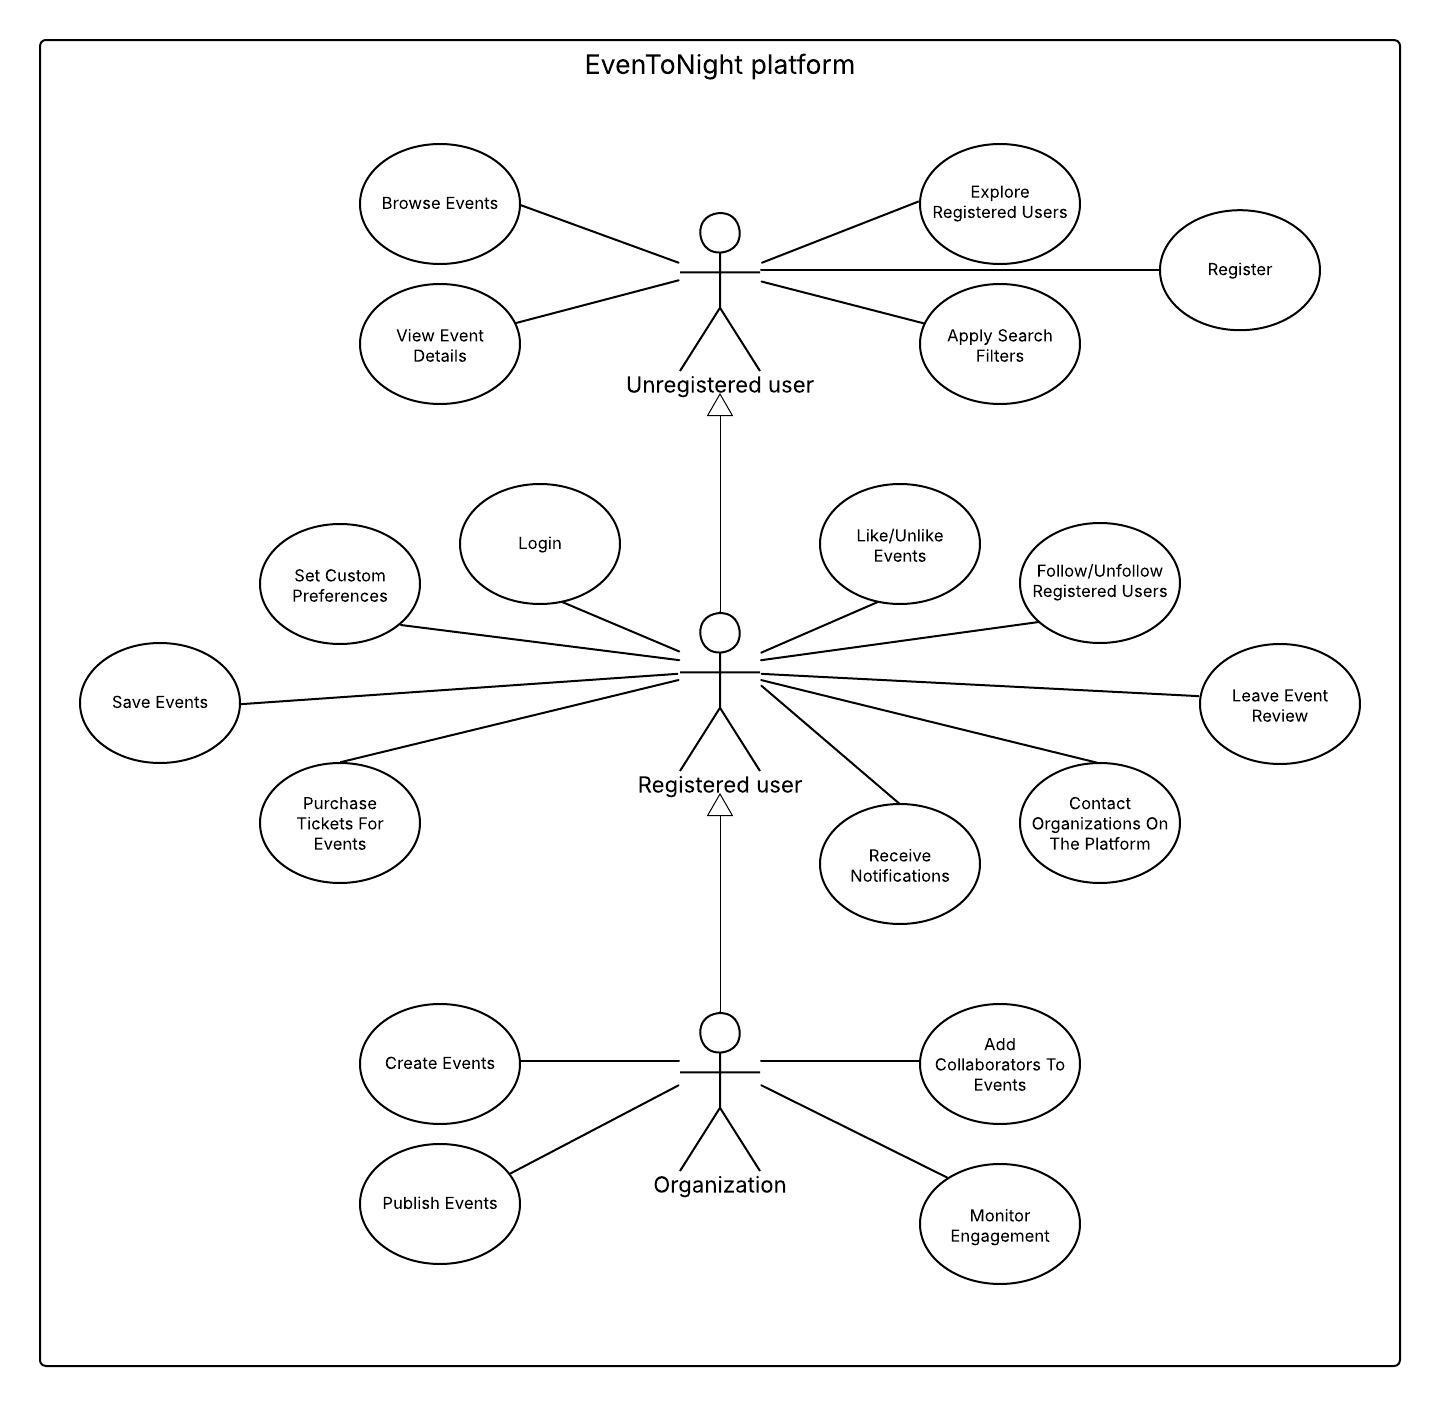
\includegraphics[width=\textwidth]{../public/case_diagram.jpeg}
  \caption{Use case diagram}
  \label{fig:case-diagram}
\end{figure}

\paragraph{Usage scenario: Browsing and filtering events as an unregistered user.}
\begin{itemize}
  \item \textbf{Actor}: Unregistered user.
  \item \textbf{Objective}: Explore events according to location and gather information without registering an account.
  \item \textbf{Main flow}:
    \begin{enumerate}
      \item The user browses the list of upcoming events.
      \item The user views event details, including poster, description, time and location.
      \item The user applies filters to find events nearby.
      \item The user searches for users registered on the platform.
    \end{enumerate}
  \item \textbf{Outcome}: The user accesses all event information without providing personal data and discovers other platform users.
\end{itemize}

\paragraph{Usage scenario: Personalized event discovery, ticket purchase and post-event review as a registered user.}
\begin{itemize}
  \item \textbf{Actor}: Registered user.
  \item \textbf{Objective}: Discover events based on personal preferences, evaluate them and purchase tickets.
  \item \textbf{Main flow}:
    \begin{enumerate}
      \item The user logs in to the EvenToNight platform.
      \item The user navigates their personalized event feed based on specified interests.
      \item The user selects an event and reads reviews on the organization's page.
      \item The user purchases tickets for the event.
    \end{enumerate}
  \item \textbf{Outcome}: The user quickly finds matching events, evaluates the organization's reliability and the purchased ticket appears on the user's personal page and can be downloaded.
  \item \textbf{Post-event action}: After attending the event, the user leaves a review on the organization's page.
\end{itemize}

\paragraph{Usage scenario: Saving events and contacting organizations as a registered user.}
\begin{itemize}
  \item \textbf{Actor}: Registered user.
  \item \textbf{Objective}: Navigate the platform, save events and contact organizations via a customized interface.
  \item \textbf{Main flow}:
    \begin{enumerate}
      \item The user logs in and navigates the platform with saved language and appearance settings.
      \item The user selects an event and saves it to their personal list.
      \item The user contacts the organization to request additional information.
    \end{enumerate}
  \item \textbf{Outcome}: Selected events are stored in the user's personal list and the user can communicate with the organization through the platform.
\end{itemize}

\paragraph{Usage scenario: Publication of events and monitoring engagement as an organization.}
\begin{itemize}
  \item \textbf{Actor}: Organization.
  \item \textbf{Objective}: Publish events and monitor user engagement.
  \item \textbf{Main flow}:
    \begin{enumerate}
      \item The user logs in and creates an event as a draft.
      \item The user adds a collaborating organization to the event.
      \item The user publishes the event.
    \end{enumerate}
  \item \textbf{Outcome}: The event is successfully published and the organization receives notifications about new followers and event likes.
\end{itemize}

\subsection{Definition of Done}

The project is considered \textit{done} when the following criteria are met:

\begin{enumerate}
  \item \textbf{Requirements fulfilled.} All main functionalities of the platform are implemented and all business and non-functional requirements are satisfied.
  \item \textbf{Testing completed.} Unit and integration tests for all services pass successfully. All API endpoints have been verified using Swagger/OpenAPI.
  \item \textbf{Deploy ready.} All services are containerized and managed via Docker Compose. The simulated distributed environment demonstrates service isolation and internal networking.
  \item \textbf{Documentation updated.} API documentation, architectural diagrams and project documentation are complete, consistent and up to date.
\end{enumerate}
